\section{Implementation}

A plugin for the Scala compiler is a separate program that can inject one or more compilation phases and alter the compiler options. In the case of ScalaDyno, we inject a single phase that takes as input the AST from the type checker phase (|typer|), traverses and cleans its erroneous statements by recursively running through all AST nodes. It also cleans up the symbol table by removing any erroneous symbol, namely any symbol whose type is either |ErrorType| or a derivate of it (e.g. |List[ErrorType]|). The final result is a pruned AST containing only references to correct symbols and symbol table which only contains correct symbols.

The normal behavior of the name resolution and type checking phases is to issue errors which prevent further compilation of the program. To achieve our goal of allowing partially correct programs to compile, we first need to prevent the compiler built-in reporter from issuing errors which makes further compilation impossible. This can be done by changing the error reporter and transforming errors into warnings. This conversion is however only done for naming and typing errors and not for errors from other phases, e.g. parsing errors as well as overriding and abstract errors which are triggered by the refcheck phase and cannot be fixed by ScalaDyno. Since errors are converted to warnings, the programmer already receives the normal feedback during compilation, in the form of warnings. During reporting, we also record the errors, which we use to later patch the tree.

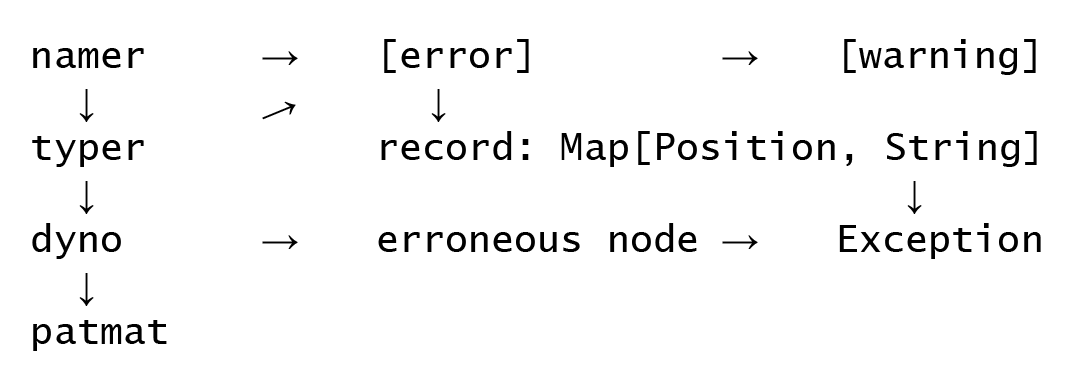
\includegraphics[width=0.9\columnwidth]{compiler_structure.png}

In the type checker, typing errors which happen on some branches in the AST propagate outwards until a stable boundary is reached. Examples of stable boundaries are the next statement in a block or the next definition in a class, trait, object or package. In order to clean up the tree, we remove the erroneous statements. Yet, as discussed before, we cannot allow the code to execute past an erroneous statement. To implement this, we actually replace erroneous statements by statements which throw exceptions. The message in the exception is the actual error output by the compiler for that particular part of the tree. This is implemented by matching source positions in the tree with source positions in the error messages. Positions are a mechanism by which the compiler records the position of each AST node in the source code. Errors also have positions attached, allowing their messages to point to the exact lines in the source code that triggered them. Therefore, based on the recorded messages and positions and the tree positions we can safely replace the tree nodes by exception-throwing statements.

There are a number of places where simply replacing an erroneous node by a statement doesn't work. Such cases are pattern matches, definitions inside classes, type-defining nodes and annotations. For these cases, we either have special rules which bubble up the statement (in the case of pattern matches) or we issue an error message that we can't properly clean up the tree and abort the compilation. While these errors could be mitigated, the additional complexity significantly burdens the plugin and does not bring significant benefit. Therefore we chose to focus on the most common errors which can easily be cleaned up.



To give a precise example for pattern matching, the following code:

\begin{lstlisting-nobreak}
object Test {
   	def main(args: Array[String]) {
   		val c = Class1(3)
	   	val ret = c match {
	   		case Class1(1) => "one"
	   		case NoSuchClass(2) => "two"
	   		case Class1(3) => "three"
	   	}
	    println(ret)
	}
}
\end{lstlisting-nobreak}

will result in a cleaned-up AST with the node after the work of the compiler plugin:

\begin{lstlisting-nobreak}
val ret: String = 'package'.this.error("
examples/Test3compilesMatch.scala:10: not found: value NoSuchClass
	   		case NoSuchClass(2) => "two"
                             ^

");
\end{lstlisting-nobreak}
